%%%%%%%%%%%%%%%%%%%%%%%%%%%%%%%%%%%%%%%%%
% University/School Laboratory Report
% LaTeX Template
% Version 3.1 (25/3/14)
%
% This template has been downloaded from:
% http://www.LaTeXTemplates.com
%
% Original author: hens

% Linux and Unix Users Group at Virginia Tech Wiki 
% (https://vtluug.org/wiki/Example_LaTeX_chem_lab_report)
%
% License:
% CC BY-NC-SA 3.0 (http://creativecommons.org/licenses/by-nc-sa/3.0/)
%
%%%%%%%%%%%%%%%%%%%%%%%%%%%%%%%%%%%%%%%%%

%----------------------------------------------------------------------------------------
%	PACKAGES AND DOCUMENT CONFIGURATIONS
%----------------------------------------------------------------------------------------

\documentclass{article}

\usepackage[version=3]{mhchem} % Package for chemical equation typesetting
\usepackage{siunitx} % Provides the \SI{}{} and \si{} command for typesetting SI units
\usepackage{graphicx} % Required for the inclusion of images
\usepackage{natbib} % Required to change bibliography style to APA
\usepackage{amsmath} % Required for some math elements 
\usepackage{german}
\usepackage[utf8]{inputenc}
\setlength\parindent{0pt} % Removes all indentation from paragraphs
\renewcommand{\labelenumi}{\alph{enumi}.} % Make numbering in the enumerate environment by letter rather than number (e.g. section 6)

%\usepackage{times} % Uncomment to use the Times New Roman font

%----------------------------------------------------------------------------------------
%	DOCUMENT INFORMATION
%----------------------------------------------------------------------------------------

\title{Physiklabor \\ Laborbericht \\ Drehmoment und Drall} % Title

\author{Daniel \textsc{Hediger} \\ Lucien \textsc{Egloff}} % Author name



\date{\today} % Date for the report

\begin{document}

\maketitle % Insert the title, author and date

\begin{center}
\begin{tabular}{l r}
Ausführungsdatum: & September 28, 2016 \\ % Date the experiment was performed
Dozent: & Dr.Ackermann % Instructor/supervisor
\end{tabular}
\end{center}
\newpage
\tableofcontents 

%----------------------------------------------------------------------------------------
%	SECTION 1
%----------------------------------------------------------------------------------------
\newpage
\section{Aufgabe 1}


Das Trägheitsmoment eines Rades soll durch das anhängen eines Gewichtes bestimmt werden.

\subsection{Grundlagen}

Das Gewicht wird durch die Erdbeschleunigung nach unten gezogen, und durch das Seil wird das Rad beschleunigt. Durch diese Beziehung kann die Winkelbeschleunigung und die Trägheit berechnet werden.

\subsection{Versuchsaufbau}
\begin{figure}[h]
\center

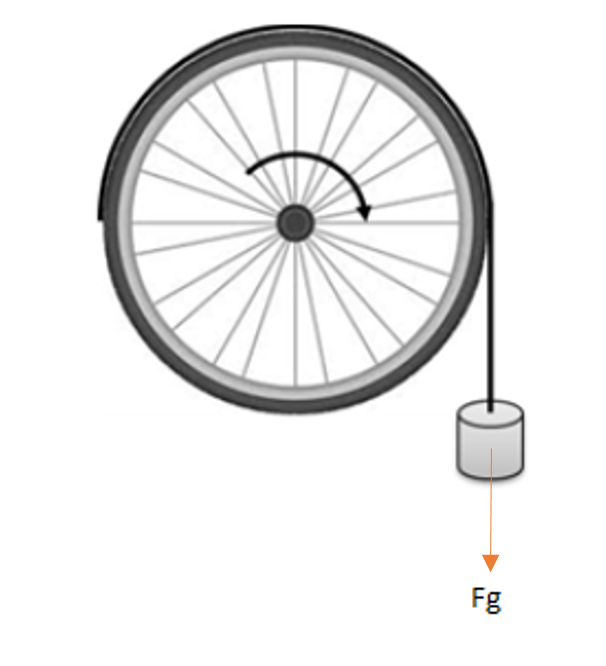
\includegraphics[scale=0.3]{Wheel.pdf} 
\caption{Fahrradrad mit angehängten Gewicht.}
\
\end{figure}
\subsection{Gemessene Grössen}
\subsection{Berechnungen}
Energieerhaltung des Systems.\\\\
$E_{rot}+E_{kin}=E_{pot}  \Rightarrow\frac{1}{2}*I*\omega+\frac{1}{2}*m*v^2=m*g*h$\\\\
Das ganze nach dem Trägheitsmoment umgestellt.\\\\
$I=\frac{-m*(v^2*2g*h)}{\omega^2} $\\\\
Das fehlende $\omega$ wurde nun Experimentell bestimmt.


\section{Aufgabe 2}
Das eigene Trägheitsmoment soll Experimentell aufgrund der Drehimpulserhaltung bestimmt werden.

\subsection{Grundlagen}
Durch die Gegebenheit der Drehzahl des Rades und dessen Trägheitsmoment, kann anhand der eigenen
Drehzahl nach dem verändern der Drehachse, das Trägheitsmoment des gesamten 
 Mensch-Hocker-Rad-Systems genähert werden.

\subsection{Versuchsaufbau}
\begin{figure}[h]
\center

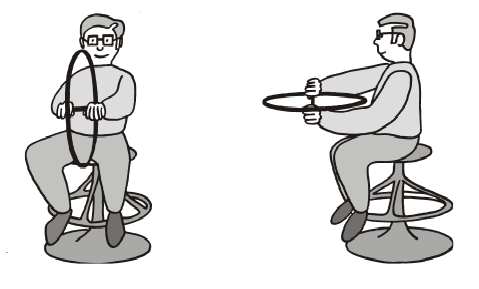
\includegraphics[scale=0.5]{Drehschemmel.pdf} 
\caption{Person mit drehendem Fahrradrad}
\
\end{figure}
\subsection{Gemessene Grössen}
\subsection{Berechnungen}
Die Grundformel
$T_p = \frac{2*\pi*(I_m+I_s)*\omega}{(m_m+m_s)*g*h} $ wird nach $I_m$(I-Mensch)umgestellt.\\\\
$I_m = \frac{g*h*(m_m+m_s)*T_p}{2*\pi*\omega}-I_s$




\section{Aufgabe 3}
Ein rotierender Kreisel wird durch das anhängen eines Gewichtes zum Präzessieren gebracht werden. Daraus lässt sich das Trägheitsmoment berechnen. 
\subsection{Grundlagen}
\subsection{Gemessene Grössen}
\subsection{Berechnungen}
\subsection{Schlussfolgerung}

\section{Aufgabe 4}
Der Drallsatz soll durch das einwirken einer horizontalen Kraft bestimmt werden.
\subsection{Grundlagen}
Der Kreisel wird beschleunigt und anschliessend mit einer Horizontalen Kraft beeinflusst. Dadurch 
beginnt er sich zu drehen, und die Zeit die er für $90^\circ$ benötigt wird gemessen. 
Anschliessend werden wir mit Hilfe des Drallsatzes, der gemessenen Werte und des 
Trägheitsmoments die Kraft welche wir aufwendeten berechnen und auf Übereinstimmung 
überprüfen. 

\subsection{Berechnungen}
$F_{Zug}=\frac{I_{Kreisel}*2*\pi*n_{Kreisel}}{T_{90^\circ }*d*60}$
\subsection{Schlussfolgerung}

\section{Aufgabe 5}

Die zeitliche Abnahme der Rotationsfrequenz des Rades und des Kreisels aufgrund von
Reibung soll bestimmt werden.
\subsection{Grundlagen}
\subsection{Versuchsaufbau}
\subsection{Gemessene Grössen}
\subsection{Schlussfolgerung}
\end{document}